% Source-coordinate reconstruction. Edit named defaults or copy this entire composition.
\studiodeclarefield{graphic-1}{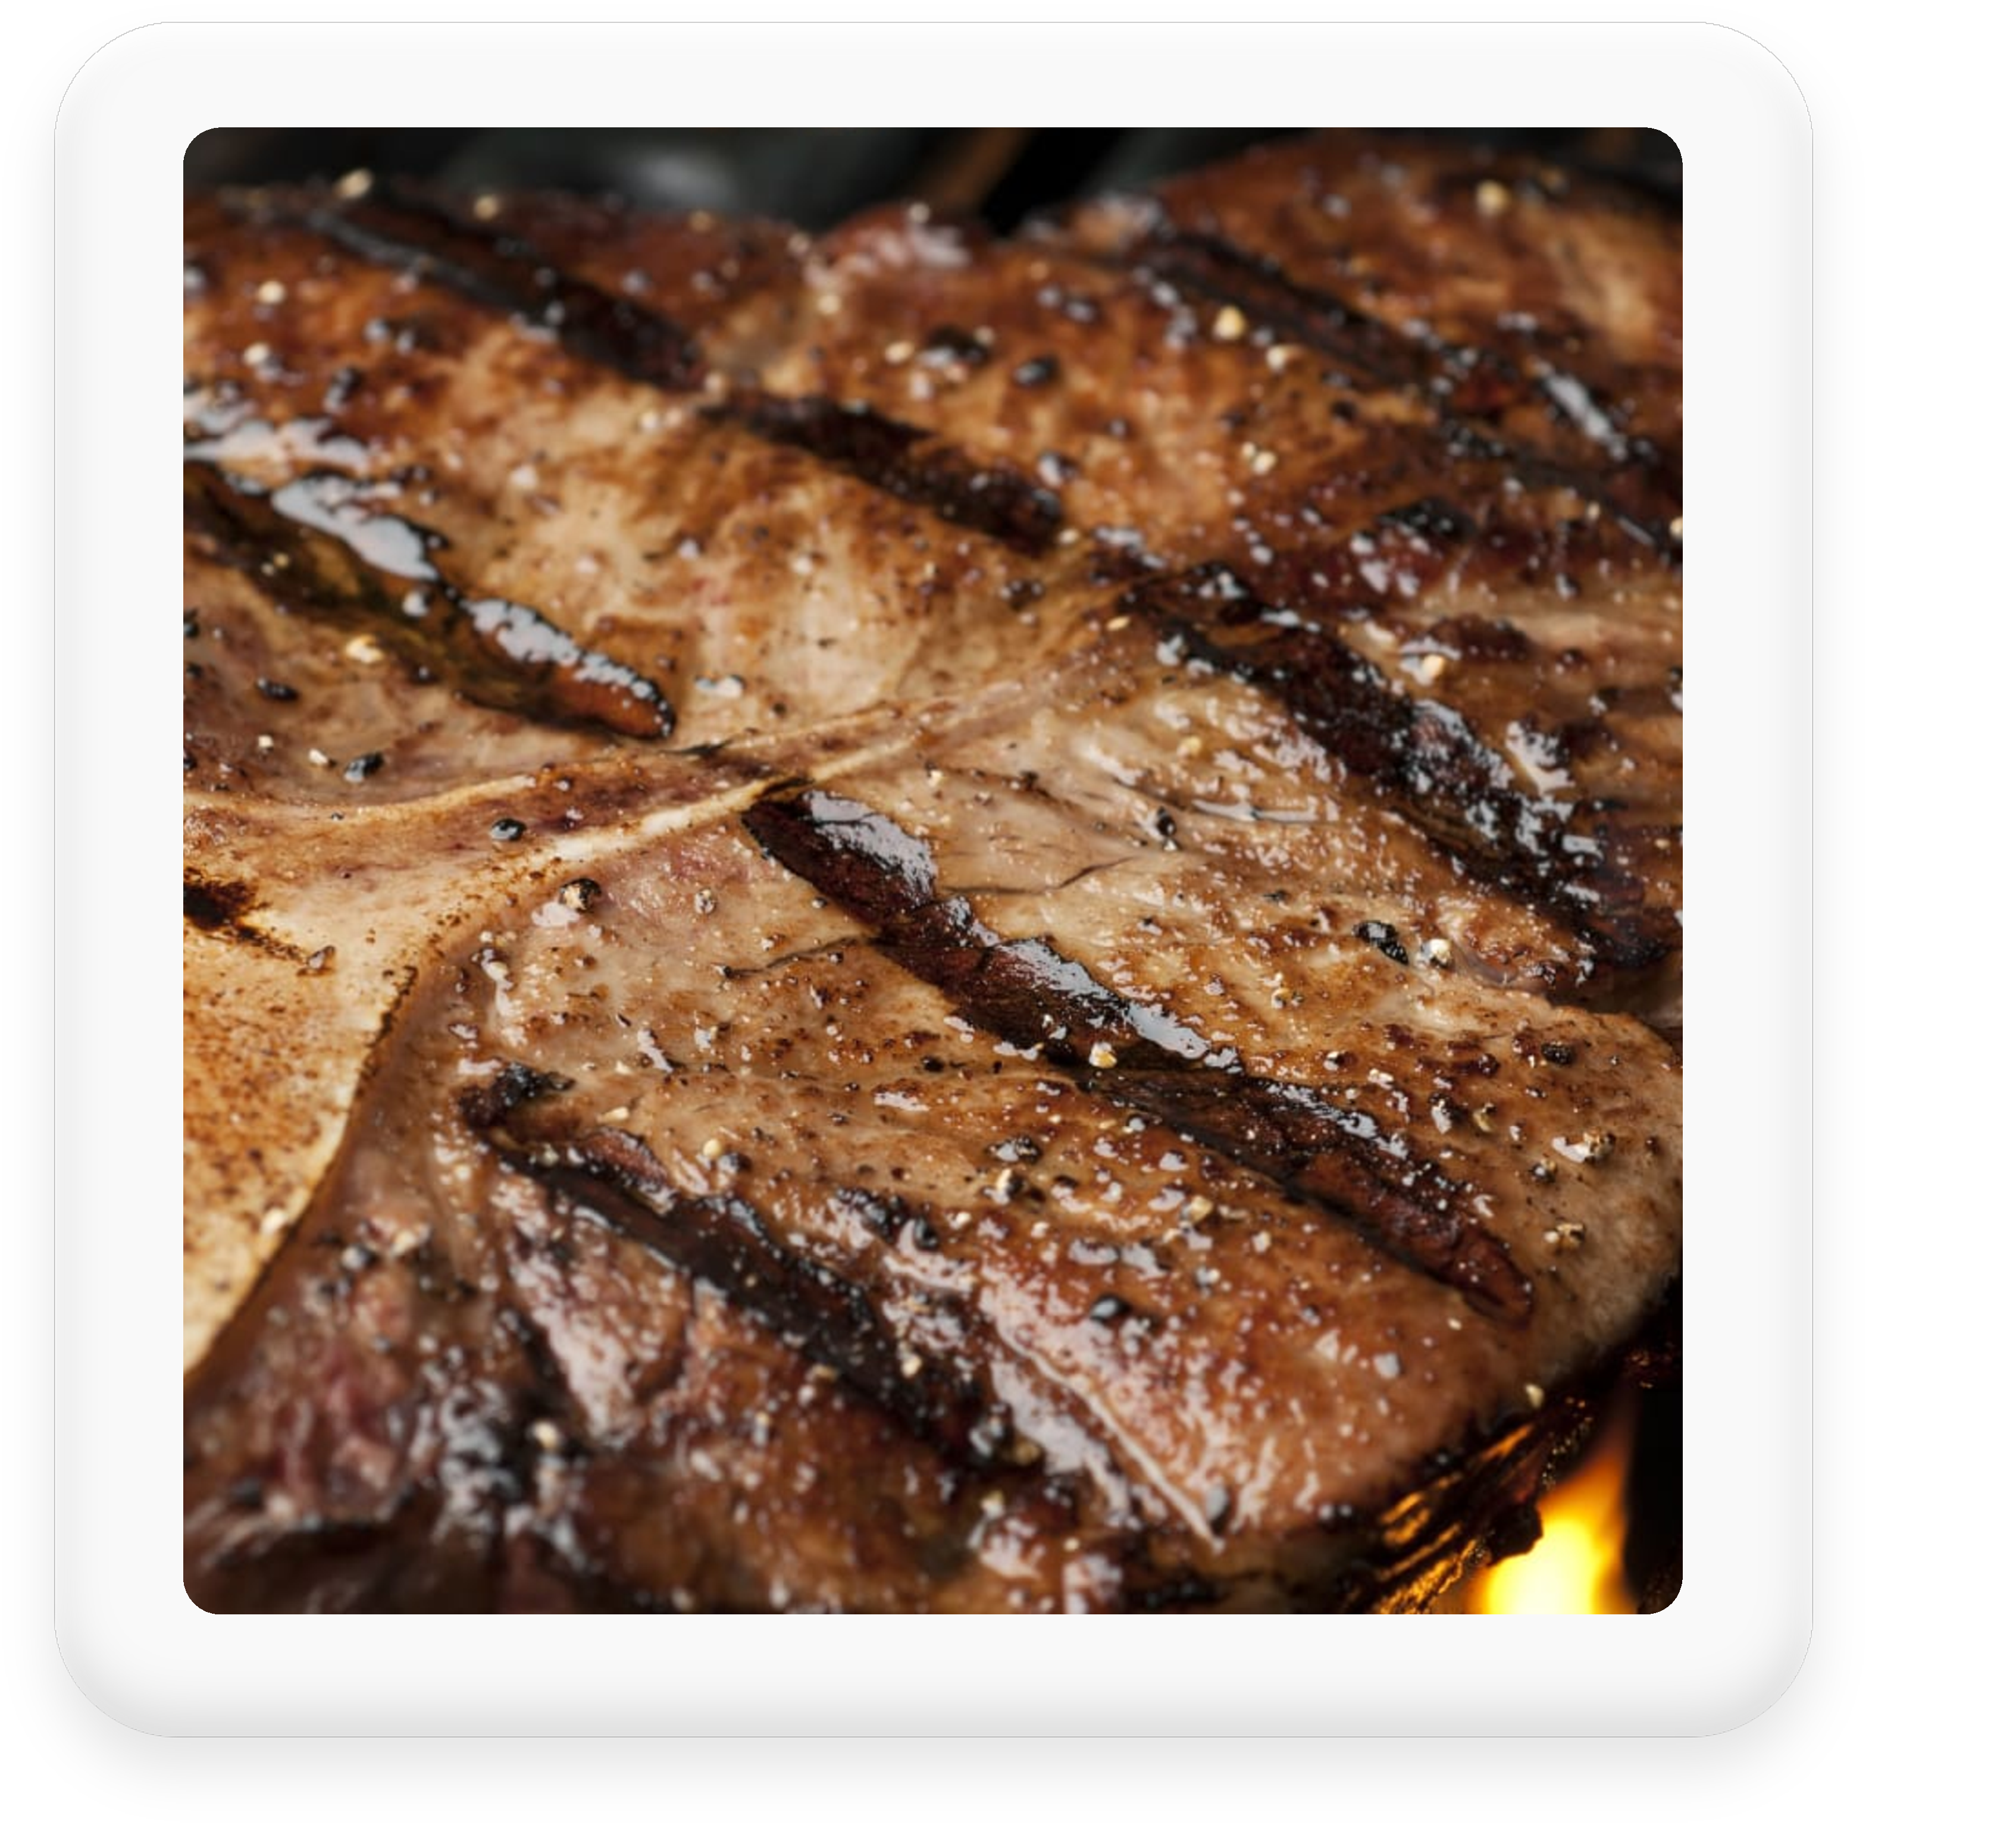
\includegraphics[width=1626\studiounit]{images/studio/collection/figma-0620-part-01.pdf}}
\studiodeclarefield{title}{``Rules without rulers''}
\studioapplyfields
\studiomeasuredcanvas{3556}{2000}{photo-center-two-icons}{studio-paper}{
\studiomeasuredtext{title}{1177.02}{227.047}{1202.96}{150.188}{112.735}{130.772}{\color{bitpolito}\bfseries\centering}{\studiofield{title}}
\studiographfield{graphic-1}{1025}{405}{1626}{1472}{}{}
\path[fill=bitpolito,draw=none,line width=1\studiounit] (433.323,1179.35)--(452.793,1179.35)--(452.793,1199)--(433.323,1199)--(433.323,1179.35)--cycle;
\path[fill=bitpolito,draw=none,line width=1\studiounit] (426.761,1198.89)--(447.522,1198.89)--(447.522,1233)--(426.761,1233)--(426.761,1198.89)--cycle;
\path[fill=bitpolito,draw=none,line width=1\studiounit] (406,1198.89)--(426.761,1198.89)--(426.761,1233)--(406,1233)--(406,1198.89)--cycle;
\path[fill=bitpolito,draw=none,line width=1\studiounit] (452.793,1061.58)--(472.371,1061.58)--(472.371,1081.23)--(452.793,1081.23)--(452.793,1061.58)--cycle;
\path[fill=bitpolito,draw=none,line width=1\studiounit] (452.793,1081.23)--(472.371,1081.23)--(472.371,1100.77)--(452.793,1100.77)--(452.793,1081.23)--cycle;
\path[fill=bitpolito,draw=none,line width=1\studiounit] (452.793,1179.35)--(472.371,1179.35)--(472.371,1199)--(452.793,1199)--(452.793,1179.35)--cycle;
\path[fill=bitpolito,draw=none,line width=1\studiounit] (447.522,1198.89)--(468.39,1198.89)--(468.39,1233)--(447.522,1233)--(447.522,1198.89)--cycle;
\path[fill=bitpolito,draw=none,line width=1\studiounit] (472.371,1002.65)--(491.948,1002.65)--(491.948,1022.29)--(472.371,1022.29)--(472.371,1002.65)--cycle;
\path[fill=bitpolito,draw=none,line width=1\studiounit] (472.371,1022.29)--(491.948,1022.29)--(491.948,1041.94)--(472.371,1041.94)--(472.371,1022.29)--cycle;
\path[fill=bitpolito,draw=none,line width=1\studiounit] (472.371,1041.94)--(491.948,1041.94)--(491.948,1061.58)--(472.371,1061.58)--(472.371,1041.94)--cycle;
\path[fill=bitpolito,draw=none,line width=1\studiounit] (472.371,1061.58)--(491.948,1061.58)--(491.948,1081.23)--(472.371,1081.23)--(472.371,1061.58)--cycle;
\path[fill=bitpolito,draw=none,line width=1\studiounit] (472.371,1081.23)--(491.948,1081.23)--(491.948,1100.77)--(472.371,1100.77)--(472.371,1081.23)--cycle;
\path[fill=bitpolito,draw=none,line width=1\studiounit] (472.371,1100.77)--(491.948,1100.77)--(491.948,1120.41)--(472.371,1120.41)--(472.371,1100.77)--cycle;
\path[fill=bitpolito,draw=none,line width=1\studiounit] (472.371,1159.71)--(491.948,1159.71)--(491.948,1179.35)--(472.371,1179.35)--(472.371,1159.71)--cycle;
\path[fill=bitpolito,draw=none,line width=1\studiounit] (472.371,1179.35)--(491.948,1179.35)--(491.948,1199)--(472.371,1199)--(472.371,1179.35)--cycle;
\path[fill=bitpolito,draw=none,line width=1\studiounit] (468.39,1198.89)--(489.367,1198.89)--(489.367,1233)--(468.39,1233)--(468.39,1198.89)--cycle;
\path[fill=bitpolito,draw=none,line width=1\studiounit] (491.948,983)--(511.526,983)--(511.526,1002.65)--(491.948,1002.65)--(491.948,983)--cycle;
\path[fill=bitpolito,draw=none,line width=1\studiounit] (491.948,1002.65)--(511.526,1002.65)--(511.526,1022.29)--(491.948,1022.29)--(491.948,1002.65)--cycle;
\path[fill=bitpolito,draw=none,line width=1\studiounit] (491.948,1022.29)--(511.526,1022.29)--(511.526,1041.94)--(491.948,1041.94)--(491.948,1022.29)--cycle;
\path[fill=bitpolito,draw=none,line width=1\studiounit] (491.948,1120.41)--(511.526,1120.41)--(511.526,1140.06)--(491.948,1140.06)--(491.948,1120.41)--cycle;
\path[fill=bitpolito,draw=none,line width=1\studiounit] (491.948,1159.71)--(511.526,1159.71)--(511.526,1179.35)--(491.948,1179.35)--(491.948,1159.71)--cycle;
\path[fill=bitpolito,draw=none,line width=1\studiounit] (491.948,1179.35)--(511.526,1179.35)--(511.526,1199)--(491.948,1199)--(491.948,1179.35)--cycle;
\path[fill=bitpolito,draw=none,line width=1\studiounit] (489.367,1198.89)--(510.235,1198.89)--(510.235,1233)--(489.367,1233)--(489.367,1198.89)--cycle;
\path[fill=bitpolito,draw=none,line width=1\studiounit] (511.526,983)--(531.104,983)--(531.104,1002.65)--(511.526,1002.65)--(511.526,983)--cycle;
\path[fill=bitpolito,draw=none,line width=1\studiounit] (511.526,1002.65)--(531.104,1002.65)--(531.104,1022.29)--(511.526,1022.29)--(511.526,1002.65)--cycle;
\path[fill=bitpolito,draw=none,line width=1\studiounit] (511.526,1022.29)--(531.104,1022.29)--(531.104,1041.94)--(511.526,1041.94)--(511.526,1022.29)--cycle;
\path[fill=bitpolito,draw=none,line width=1\studiounit] (511.526,1140.06)--(531.104,1140.06)--(531.104,1159.71)--(511.526,1159.71)--(511.526,1140.06)--cycle;
\path[fill=bitpolito,draw=none,line width=1\studiounit] (511.526,1179.35)--(531.104,1179.35)--(531.104,1199)--(511.526,1199)--(511.526,1179.35)--cycle;
\path[fill=bitpolito,draw=none,line width=1\studiounit] (510.235,1198.89)--(531.104,1198.89)--(531.104,1233)--(510.235,1233)--(510.235,1198.89)--cycle;
\path[fill=bitpolito,draw=none,line width=1\studiounit] (531.104,983)--(550.681,983)--(550.681,1002.65)--(531.104,1002.65)--(531.104,983)--cycle;
\path[fill=bitpolito,draw=none,line width=1\studiounit] (531.104,1002.65)--(550.681,1002.65)--(550.681,1022.29)--(531.104,1022.29)--(531.104,1002.65)--cycle;
\path[fill=bitpolito,draw=none,line width=1\studiounit] (531.104,1022.29)--(550.681,1022.29)--(550.681,1041.94)--(531.104,1041.94)--(531.104,1022.29)--cycle;
\path[fill=bitpolito,draw=none,line width=1\studiounit] (531.104,1140.06)--(550.681,1140.06)--(550.681,1159.71)--(531.104,1159.71)--(531.104,1140.06)--cycle;
\path[fill=bitpolito,draw=none,line width=1\studiounit] (550.681,983)--(570.259,983)--(570.259,1002.65)--(550.681,1002.65)--(550.681,983)--cycle;
\path[fill=bitpolito,draw=none,line width=1\studiounit] (550.681,1002.65)--(570.259,1002.65)--(570.259,1022.29)--(550.681,1022.29)--(550.681,1002.65)--cycle;
\path[fill=bitpolito,draw=none,line width=1\studiounit] (550.681,1140.06)--(570.259,1140.06)--(570.259,1159.71)--(550.681,1159.71)--(550.681,1140.06)--cycle;
\path[fill=bitpolito,draw=none,line width=1\studiounit] (550.681,1179.35)--(570.259,1179.35)--(570.259,1199)--(550.681,1199)--(550.681,1179.35)--cycle;
\path[fill=bitpolito,draw=none,line width=1\studiounit] (550.681,1198.89)--(571.55,1198.89)--(571.55,1233)--(550.681,1233)--(550.681,1198.89)--cycle;
\path[fill=bitpolito,draw=none,line width=1\studiounit] (570.259,983)--(589.837,983)--(589.837,1002.65)--(570.259,1002.65)--(570.259,983)--cycle;
\path[fill=bitpolito,draw=none,line width=1\studiounit] (570.259,1022.29)--(589.837,1022.29)--(589.837,1041.94)--(570.259,1041.94)--(570.259,1022.29)--cycle;
\path[fill=bitpolito,draw=none,line width=1\studiounit] (570.259,1120.41)--(589.837,1120.41)--(589.837,1140.06)--(570.259,1140.06)--(570.259,1120.41)--cycle;
\path[fill=bitpolito,draw=none,line width=1\studiounit] (570.259,1159.71)--(589.837,1159.71)--(589.837,1179.35)--(570.259,1179.35)--(570.259,1159.71)--cycle;
\path[fill=bitpolito,draw=none,line width=1\studiounit] (570.259,1179.35)--(589.837,1179.35)--(589.837,1199)--(570.259,1199)--(570.259,1179.35)--cycle;
\path[fill=bitpolito,draw=none,line width=1\studiounit] (571.55,1198.89)--(592.418,1198.89)--(592.418,1233)--(571.55,1233)--(571.55,1198.89)--cycle;
\path[fill=bitpolito,draw=none,line width=1\studiounit] (589.837,1002.65)--(609.414,1002.65)--(609.414,1022.29)--(589.837,1022.29)--(589.837,1002.65)--cycle;
\path[fill=bitpolito,draw=none,line width=1\studiounit] (589.837,1022.29)--(609.414,1022.29)--(609.414,1041.94)--(589.837,1041.94)--(589.837,1022.29)--cycle;
\path[fill=bitpolito,draw=none,line width=1\studiounit] (589.837,1041.94)--(609.414,1041.94)--(609.414,1061.58)--(589.837,1061.58)--(589.837,1041.94)--cycle;
\path[fill=bitpolito,draw=none,line width=1\studiounit] (589.837,1061.58)--(609.414,1061.58)--(609.414,1081.23)--(589.837,1081.23)--(589.837,1061.58)--cycle;
\path[fill=bitpolito,draw=none,line width=1\studiounit] (589.837,1081.23)--(609.414,1081.23)--(609.414,1100.77)--(589.837,1100.77)--(589.837,1081.23)--cycle;
\path[fill=bitpolito,draw=none,line width=1\studiounit] (589.837,1100.77)--(609.414,1100.77)--(609.414,1120.41)--(589.837,1120.41)--(589.837,1100.77)--cycle;
\path[fill=bitpolito,draw=none,line width=1\studiounit] (589.837,1159.71)--(609.414,1159.71)--(609.414,1179.35)--(589.837,1179.35)--(589.837,1159.71)--cycle;
\path[fill=bitpolito,draw=none,line width=1\studiounit] (589.837,1179.35)--(609.414,1179.35)--(609.414,1199)--(589.837,1199)--(589.837,1179.35)--cycle;
\path[fill=bitpolito,draw=none,line width=1\studiounit] (592.418,1198.89)--(613.287,1198.89)--(613.287,1233)--(592.418,1233)--(592.418,1198.89)--cycle;
\path[fill=bitpolito,draw=none,line width=1\studiounit] (609.414,1061.58)--(628.992,1061.58)--(628.992,1081.23)--(609.414,1081.23)--(609.414,1061.58)--cycle;
\path[fill=bitpolito,draw=none,line width=1\studiounit] (609.414,1081.23)--(628.992,1081.23)--(628.992,1100.77)--(609.414,1100.77)--(609.414,1081.23)--cycle;
\path[fill=bitpolito,draw=none,line width=1\studiounit] (609.414,1179.35)--(628.992,1179.35)--(628.992,1199)--(609.414,1199)--(609.414,1179.35)--cycle;
\path[fill=bitpolito,draw=none,line width=1\studiounit] (613.287,1198.89)--(634.263,1198.89)--(634.263,1233)--(613.287,1233)--(613.287,1198.89)--cycle;
\path[fill=bitpolito,draw=none,line width=1\studiounit] (628.992,1179.35)--(648.57,1179.35)--(648.57,1199)--(628.992,1199)--(628.992,1179.35)--cycle;
\path[fill=bitpolito,draw=none,line width=1\studiounit] (634.263,1198.89)--(655.131,1198.89)--(655.131,1233)--(634.263,1233)--(634.263,1198.89)--cycle;
\path[fill=bitpolito,draw=none,line width=1\studiounit] (655.131,1198.89)--(676,1198.89)--(676,1233)--(655.131,1233)--(655.131,1198.89)--cycle;
\path[fill=bitpolito,draw=none,line width=1\studiounit] (2900,1216.36)--(2922.73,1216.36)--(2922.73,1239)--(2900,1239)--(2900,1216.36)--cycle;
\path[fill=bitpolito,draw=none,line width=1\studiounit] (2922.73,1080.55)--(2945.45,1080.55)--(2945.45,1103.18)--(2922.73,1103.18)--(2922.73,1080.55)--cycle;
\path[fill=bitpolito,draw=none,line width=1\studiounit] (2922.73,1103.18)--(2945.45,1103.18)--(2945.45,1125.82)--(2922.73,1125.82)--(2922.73,1103.18)--cycle;
\path[fill=bitpolito,draw=none,line width=1\studiounit] (2922.73,1125.82)--(2945.45,1125.82)--(2945.45,1148.45)--(2922.73,1148.45)--(2922.73,1125.82)--cycle;
\path[fill=bitpolito,draw=none,line width=1\studiounit] (2922.73,1148.45)--(2945.45,1148.45)--(2945.45,1171.09)--(2922.73,1171.09)--(2922.73,1148.45)--cycle;
\path[fill=bitpolito,draw=none,line width=1\studiounit] (2900,1148.45)--(2922.73,1148.45)--(2922.73,1171.09)--(2900,1171.09)--(2900,1148.45)--cycle;
\path[fill=bitpolito,draw=none,line width=1\studiounit] (2900,1125.82)--(2922.73,1125.82)--(2922.73,1148.45)--(2900,1148.45)--(2900,1125.82)--cycle;
\path[fill=bitpolito,draw=none,line width=1\studiounit] (2945.45,1148.45)--(2968.18,1148.45)--(2968.18,1171.09)--(2945.45,1171.09)--(2945.45,1148.45)--cycle;
\path[fill=bitpolito,draw=none,line width=1\studiounit] (2922.73,1216.36)--(2945.45,1216.36)--(2945.45,1239)--(2922.73,1239)--(2922.73,1216.36)--cycle;
\path[fill=bitpolito,draw=none,line width=1\studiounit] (2945.45,1012.64)--(2968.18,1012.64)--(2968.18,1035.27)--(2945.45,1035.27)--(2945.45,1012.64)--cycle;
\path[fill=bitpolito,draw=none,line width=1\studiounit] (2945.45,1035.27)--(2968.18,1035.27)--(2968.18,1057.91)--(2945.45,1057.91)--(2945.45,1035.27)--cycle;
\path[fill=bitpolito,draw=none,line width=1\studiounit] (2945.45,1057.91)--(2968.18,1057.91)--(2968.18,1080.55)--(2945.45,1080.55)--(2945.45,1057.91)--cycle;
\path[fill=bitpolito,draw=none,line width=1\studiounit] (2945.45,1080.55)--(2968.18,1080.55)--(2968.18,1103.18)--(2945.45,1103.18)--(2945.45,1080.55)--cycle;
\path[fill=bitpolito,draw=none,line width=1\studiounit] (2945.45,1103.18)--(2968.18,1103.18)--(2968.18,1125.82)--(2945.45,1125.82)--(2945.45,1103.18)--cycle;
\path[fill=bitpolito,draw=none,line width=1\studiounit] (2945.45,1125.82)--(2968.18,1125.82)--(2968.18,1148.45)--(2945.45,1148.45)--(2945.45,1125.82)--cycle;
\path[fill=bitpolito,draw=none,line width=1\studiounit] (2945.45,1193.73)--(2968.18,1193.73)--(2968.18,1216.36)--(2945.45,1216.36)--(2945.45,1193.73)--cycle;
\path[fill=bitpolito,draw=none,line width=1\studiounit] (2945.45,1216.36)--(2968.18,1216.36)--(2968.18,1239)--(2945.45,1239)--(2945.45,1216.36)--cycle;
\path[fill=bitpolito,draw=none,line width=1\studiounit] (2968.18,990)--(2990.91,990)--(2990.91,1012.64)--(2968.18,1012.64)--(2968.18,990)--cycle;
\path[fill=bitpolito,draw=none,line width=1\studiounit] (2968.18,1012.64)--(2990.91,1012.64)--(2990.91,1035.27)--(2968.18,1035.27)--(2968.18,1012.64)--cycle;
\path[fill=bitpolito,draw=none,line width=1\studiounit] (2968.18,1035.27)--(2990.91,1035.27)--(2990.91,1057.91)--(2968.18,1057.91)--(2968.18,1035.27)--cycle;
\path[fill=bitpolito,draw=none,line width=1\studiounit] (2968.18,1057.91)--(2990.91,1057.91)--(2990.91,1080.55)--(2968.18,1080.55)--(2968.18,1057.91)--cycle;
\path[fill=bitpolito,draw=none,line width=1\studiounit] (2922.73,1057.91)--(2945.45,1057.91)--(2945.45,1080.55)--(2922.73,1080.55)--(2922.73,1057.91)--cycle;
\path[fill=bitpolito,draw=none,line width=1\studiounit] (3104.55,1057.91)--(3127.27,1057.91)--(3127.27,1080.55)--(3104.55,1080.55)--(3104.55,1057.91)--cycle;
\path[fill=bitpolito,draw=none,line width=1\studiounit] (2968.18,1148.45)--(2990.91,1148.45)--(2990.91,1171.09)--(2968.18,1171.09)--(2968.18,1148.45)--cycle;
\path[fill=bitpolito,draw=none,line width=1\studiounit] (2968.18,1193.73)--(2990.91,1193.73)--(2990.91,1216.36)--(2968.18,1216.36)--(2968.18,1193.73)--cycle;
\path[fill=bitpolito,draw=none,line width=1\studiounit] (2968.18,1216.36)--(2990.91,1216.36)--(2990.91,1239)--(2968.18,1239)--(2968.18,1216.36)--cycle;
\path[fill=bitpolito,draw=none,line width=1\studiounit] (2990.91,990)--(3013.64,990)--(3013.64,1012.64)--(2990.91,1012.64)--(2990.91,990)--cycle;
\path[fill=bitpolito,draw=none,line width=1\studiounit] (2990.91,1012.64)--(3013.64,1012.64)--(3013.64,1035.27)--(2990.91,1035.27)--(2990.91,1012.64)--cycle;
\path[fill=bitpolito,draw=none,line width=1\studiounit] (2990.91,1035.27)--(3013.64,1035.27)--(3013.64,1057.91)--(2990.91,1057.91)--(2990.91,1035.27)--cycle;
\path[fill=bitpolito,draw=none,line width=1\studiounit] (2990.91,1171.09)--(3013.64,1171.09)--(3013.64,1193.73)--(2990.91,1193.73)--(2990.91,1171.09)--cycle;
\path[fill=bitpolito,draw=none,line width=1\studiounit] (2990.91,1216.36)--(3013.64,1216.36)--(3013.64,1239)--(2990.91,1239)--(2990.91,1216.36)--cycle;
\path[fill=bitpolito,draw=none,line width=1\studiounit] (3013.64,990)--(3036.36,990)--(3036.36,1012.64)--(3013.64,1012.64)--(3013.64,990)--cycle;
\path[fill=bitpolito,draw=none,line width=1\studiounit] (3013.64,1012.64)--(3036.36,1012.64)--(3036.36,1035.27)--(3013.64,1035.27)--(3013.64,1012.64)--cycle;
\path[fill=bitpolito,draw=none,line width=1\studiounit] (3013.64,1035.27)--(3036.36,1035.27)--(3036.36,1057.91)--(3013.64,1057.91)--(3013.64,1035.27)--cycle;
\path[fill=bitpolito,draw=none,line width=1\studiounit] (3013.64,1171.09)--(3036.36,1171.09)--(3036.36,1193.73)--(3013.64,1193.73)--(3013.64,1171.09)--cycle;
\path[fill=bitpolito,draw=none,line width=1\studiounit] (3036.36,990)--(3059.09,990)--(3059.09,1012.64)--(3036.36,1012.64)--(3036.36,990)--cycle;
\path[fill=bitpolito,draw=none,line width=1\studiounit] (3036.36,1012.64)--(3059.09,1012.64)--(3059.09,1035.27)--(3036.36,1035.27)--(3036.36,1012.64)--cycle;
\path[fill=bitpolito,draw=none,line width=1\studiounit] (3036.36,1171.09)--(3059.09,1171.09)--(3059.09,1193.73)--(3036.36,1193.73)--(3036.36,1171.09)--cycle;
\path[fill=bitpolito,draw=none,line width=1\studiounit] (3036.36,1216.36)--(3059.09,1216.36)--(3059.09,1239)--(3036.36,1239)--(3036.36,1216.36)--cycle;
\path[fill=bitpolito,draw=none,line width=1\studiounit] (3059.09,990)--(3081.82,990)--(3081.82,1012.64)--(3059.09,1012.64)--(3059.09,990)--cycle;
\path[fill=bitpolito,draw=none,line width=1\studiounit] (3059.09,1035.27)--(3081.82,1035.27)--(3081.82,1057.91)--(3059.09,1057.91)--(3059.09,1035.27)--cycle;
\path[fill=bitpolito,draw=none,line width=1\studiounit] (3059.09,1148.45)--(3081.82,1148.45)--(3081.82,1171.09)--(3059.09,1171.09)--(3059.09,1148.45)--cycle;
\path[fill=bitpolito,draw=none,line width=1\studiounit] (3059.09,1193.73)--(3081.82,1193.73)--(3081.82,1216.36)--(3059.09,1216.36)--(3059.09,1193.73)--cycle;
\path[fill=bitpolito,draw=none,line width=1\studiounit] (3059.09,1216.36)--(3081.82,1216.36)--(3081.82,1239)--(3059.09,1239)--(3059.09,1216.36)--cycle;
\path[fill=bitpolito,draw=none,line width=1\studiounit] (3081.82,1012.64)--(3104.55,1012.64)--(3104.55,1035.27)--(3081.82,1035.27)--(3081.82,1012.64)--cycle;
\path[fill=bitpolito,draw=none,line width=1\studiounit] (3081.82,1035.27)--(3104.55,1035.27)--(3104.55,1057.91)--(3081.82,1057.91)--(3081.82,1035.27)--cycle;
\path[fill=bitpolito,draw=none,line width=1\studiounit] (3081.82,1057.91)--(3104.55,1057.91)--(3104.55,1080.55)--(3081.82,1080.55)--(3081.82,1057.91)--cycle;
\path[fill=bitpolito,draw=none,line width=1\studiounit] (3081.82,1080.55)--(3104.55,1080.55)--(3104.55,1103.18)--(3081.82,1103.18)--(3081.82,1080.55)--cycle;
\path[fill=bitpolito,draw=none,line width=1\studiounit] (3081.82,1103.18)--(3104.55,1103.18)--(3104.55,1125.82)--(3081.82,1125.82)--(3081.82,1103.18)--cycle;
\path[fill=bitpolito,draw=none,line width=1\studiounit] (3081.82,1125.82)--(3104.55,1125.82)--(3104.55,1148.45)--(3081.82,1148.45)--(3081.82,1125.82)--cycle;
\path[fill=bitpolito,draw=none,line width=1\studiounit] (3081.82,1148.45)--(3104.55,1148.45)--(3104.55,1171.09)--(3081.82,1171.09)--(3081.82,1148.45)--cycle;
\path[fill=bitpolito,draw=none,line width=1\studiounit] (3081.82,1193.73)--(3104.55,1193.73)--(3104.55,1216.36)--(3081.82,1216.36)--(3081.82,1193.73)--cycle;
\path[fill=bitpolito,draw=none,line width=1\studiounit] (3081.82,1216.36)--(3104.55,1216.36)--(3104.55,1239)--(3081.82,1239)--(3081.82,1216.36)--cycle;
\path[fill=bitpolito,draw=none,line width=1\studiounit] (3104.55,1080.55)--(3127.27,1080.55)--(3127.27,1103.18)--(3104.55,1103.18)--(3104.55,1080.55)--cycle;
\path[fill=bitpolito,draw=none,line width=1\studiounit] (3104.55,1103.18)--(3127.27,1103.18)--(3127.27,1125.82)--(3104.55,1125.82)--(3104.55,1103.18)--cycle;
\path[fill=bitpolito,draw=none,line width=1\studiounit] (3104.55,1125.82)--(3127.27,1125.82)--(3127.27,1148.45)--(3104.55,1148.45)--(3104.55,1125.82)--cycle;
\path[fill=bitpolito,draw=none,line width=1\studiounit] (3127.27,1125.82)--(3150,1125.82)--(3150,1148.45)--(3127.27,1148.45)--(3127.27,1125.82)--cycle;
\path[fill=bitpolito,draw=none,line width=1\studiounit] (3104.55,1148.45)--(3127.27,1148.45)--(3127.27,1171.09)--(3104.55,1171.09)--(3104.55,1148.45)--cycle;
\path[fill=bitpolito,draw=none,line width=1\studiounit] (3127.27,1148.45)--(3150,1148.45)--(3150,1171.09)--(3127.27,1171.09)--(3127.27,1148.45)--cycle;
\path[fill=bitpolito,draw=none,line width=1\studiounit] (3104.55,1216.36)--(3127.27,1216.36)--(3127.27,1239)--(3104.55,1239)--(3104.55,1216.36)--cycle;
\path[fill=bitpolito,draw=none,line width=1\studiounit] (3127.27,1216.36)--(3150,1216.36)--(3150,1239)--(3127.27,1239)--(3127.27,1216.36)--cycle;
}
